% chapters/tikz_ch08.tex - 第 8 章插图 (TikZ 全矢量重绘)
% 图 8.1 光锥与零双特征线; 图 8.2 实主型传播估计

% ============ 图 8.1 ============
\newcommand{\drawFigEightOne}{%
\begin{tikzpicture}[scale=1.0, >=stealth, line join=round]
    % ---------- 左图: 波动算子的特征集 ----------
    \begin{scope}[shift={(0,0)}]
        \draw[->] (0.25,0.25) -- (5.9,0.25) node[right, font=\small] {$x$};
        \draw[->] (0.25,0.25) -- (0.25,5.20) node[above, font=\small] {$t$};
        % 双光锥 1
        \coordinate (P0) at (1.40,1.00);
        \draw[thick] (P0) -- ++(0.85,0.85);
        \draw[thick] (P0) -- ++(-0.85,0.85);
        \draw[thick] (P0) -- ++(0.60,-0.60);
        \draw[thick] (P0) -- ++(-0.60,-0.60);
        \fill (P0) circle (1.6pt);
        \node[below left, font=\small] at (1.42,0.96) {$(t_0,x_0)$};
        % 双光锥 2
        \coordinate (P1) at (4.40,4.00);
        \draw[thick] (P1) -- ++(0.85,0.85);
        \draw[thick] (P1) -- ++(-0.85,0.85);
        \draw[thick] (P1) -- ++(0.60,-0.60);
        \draw[thick] (P1) -- ++(-0.60,-0.60);
        \fill (P1) circle (1.6pt);
        \node[right, font=\small] at (4.46,4.02) {$(t_1,x_1)$};
        % 零双特征线上的两个点与底投影
        \coordinate (A) at (1.95,1.55);
        \coordinate (B) at (3.85,3.45);
        \fill[gray!70] (A) circle (2.2pt);
        \fill[gray!70] (B) circle (2.2pt);
        \draw[very thick, gray!70] (A) -- (B);
        \draw[densely dashed, gray] (A) -- ($(A)-(0,0.55)$);
        \draw[densely dashed, gray] (B) -- ($(B)-(0,0.55)$);
    \end{scope}
    % ---------- 右图: 乘子算子的零双特征线 ----------
    \begin{scope}[shift={(6.55,0.55)}]
        \draw[->] (0,0) -- (4.70,0) node[right, font=\small] {$\xi$};
        \node[below left, font=\small] at (0.02,-0.02) {$0$};
        \fill (1.30,0) circle (1.6pt);
        \node[below, font=\small] at (1.30,-0.06) {$\xi_0$};
        \fill[gray!70] (3.30,0) circle (2.2pt);
        \node[below, font=\small] at (3.30,-0.06) {$\xi_0+s\tilde{\xi}$};
        \draw[very thick, gray!70, ->] (1.42,0) -- (3.18,0);
        \node[above, font=\small] at (2.35,0.55) {$-\partial_x p_4(x_0)$};
        \draw[->] (2.35,0.45) -- (2.95,0.08);
        \node[above, font=\small] at (1.30,0.95) {纤维 $T^*_{x_0}\R^n$};
        \node[font=\small] at (2.35,-1.15) {$\operatorname{Char}(P_4)=\{p_4(x_0)=0,\ \xi\neq 0\}$};
    \end{scope}
\end{tikzpicture}}

% ============ 图 8.2 ============
\newcommand{\drawFigEightTwo}{%
\begin{tikzpicture}[scale=1.0, >=stealth]
    % 邻域 U
    \draw[gray, densely dashed, rounded corners=8pt] (0.20,0.35) rectangle (8.20,3.55);
    \node[gray, font=\small, anchor=north east] at (8.10,3.48) {$\mathcal{U}$};
    % 零双特征线
    \draw[very thick] (1.30,1.00) .. controls (3.20,1.05) and (5.40,2.65) .. (7.30,3.00);
    \fill (1.30,1.00) circle (1.8pt);
    \node[below left, font=\small] at (1.30,0.92) {$\gamma(0)$};
    \fill (7.30,3.00) circle (1.8pt);
    \node[above right, font=\small] at (7.32,3.06) {$\gamma(s_0)$};
    % Ell(E)
    \draw[very thick, gray!60, fill=gray!12] (1.30,1.00) ellipse (0.95 and 0.62);
    \node[font=\small] at (1.30,1.82) {$\Ell(E)$};
    % Ell(B): 沿曲线的灰带
    \draw[line width=9pt, gray!25, line cap=round] (2.35,1.02) .. controls (3.40,1.25) and (5.20,2.55) .. (6.55,2.93);
    \node[font=\small] at (4.55,1.35) {$\Ell(B)$};
    % 右侧说明
    \node[font=\small, anchor=west, align=left] at (0.40,3.15)
        {在此 $\gamma$ 的邻域内 $GPu\in H^{s-m+1}$};
    \draw[->, gray] (2.55,3.02) -- (4.10,2.72);
\end{tikzpicture}}

% ============ 图 8.3 ============
\newcommand{\drawFigEightThree}{%
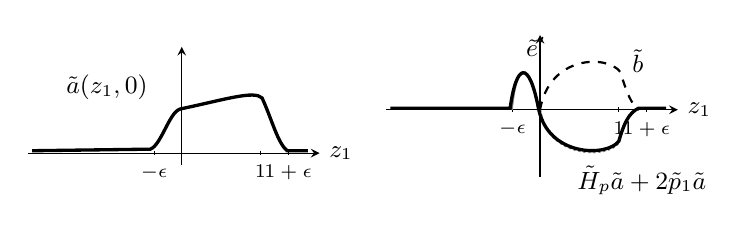
\begin{tikzpicture}[scale=1.0, >=stealth]
    % ---------- 左图: 对易子 \tilde a 的图像 ----------
    \begin{scope}[shift={(0,0)}]
        \draw[->] (-1.95,0) -- (1.75,0) node[right, font=\small] {$z_1$};
        \draw[->] (0,-0.15) -- (0,1.35);
        \foreach \x/\lab in {-0.35/{-\epsilon}, 1.0/{1}, 1.35/{1+\epsilon}}
            \draw (\x,0.03) -- (\x,-0.03) node[below, font=\scriptsize] {$\lab$};
        \draw[very thick] (-1.90,0.03) -- (-0.40,0.05)
            .. controls (-0.26,0.10) and (-0.16,0.52) .. (-0.02,0.56)
            .. controls (0.55,0.68) and (0.92,0.80) .. (1.02,0.70)
            .. controls (1.14,0.44) and (1.22,0.12) .. (1.34,0.03)
            -- (1.60,0.03);
        \node[above, font=\small] at (-0.95,0.55) {$\tilde{a}(z_1,0)$};
    \end{scope}
    % ---------- 右图: (8.46) 中的各项 ----------
    \begin{scope}[shift={(4.55,0.55)}]
        \draw[->] (-1.95,0) -- (1.75,0) node[right, font=\small] {$z_1$};
        \draw[->] (0,-0.85) -- (0,0.95);
        \foreach \x/\lab in {-0.35/{-\epsilon}, 1.0/{1}, 1.35/{1+\epsilon}}
            \draw (\x,0.03) -- (\x,-0.03) node[below, font=\scriptsize] {$\lab$};
        % \tilde e' 的正尖峰
        \draw[thick, gray] (-0.36,0) .. controls (-0.30,0.62) and (-0.14,0.66) .. (-0.02,0);
        % -\tilde b^2 的负平台
        \draw[thick, gray, densely dotted] (0,0) .. controls (0.10,-0.62) and (0.85,-0.62) .. (1.00,-0.42)
            .. controls (1.06,-0.18) and (1.12,-0.05) .. (1.22,0);
        % 合成曲线 H_p a + 2 p_1 a
        \draw[very thick] (-1.90,0.02) -- (-0.38,0.02)
            .. controls (-0.30,0.60) and (-0.14,0.64) .. (-0.02,0.02)
            .. controls (0.10,-0.60) and (0.85,-0.60) .. (1.00,-0.40)
            .. controls (1.07,-0.16) and (1.13,-0.04) .. (1.25,0.02)
            -- (1.60,0.02);
        % \tilde b
        \draw[thick, dashed] (0,0) .. controls (0.12,0.70) and (0.86,0.70) .. (1.02,0.48)
            .. controls (1.10,0.22) and (1.16,0.06) .. (1.26,0);
        \node[font=\small, anchor=west] at (0.35,-0.90) {$\tilde{H}_p\tilde{a}+2\tilde{p}_1\tilde{a}$};
        \node[font=\small, anchor=west] at (1.05,0.62) {$\tilde{b}$};
        \node[font=\small, anchor=west] at (-0.30,0.80) {$\tilde{e}'$};
    \end{scope}
\end{tikzpicture}}

% ============ 图 8.4 ============
\newcommand{\drawFigEightFour}{%
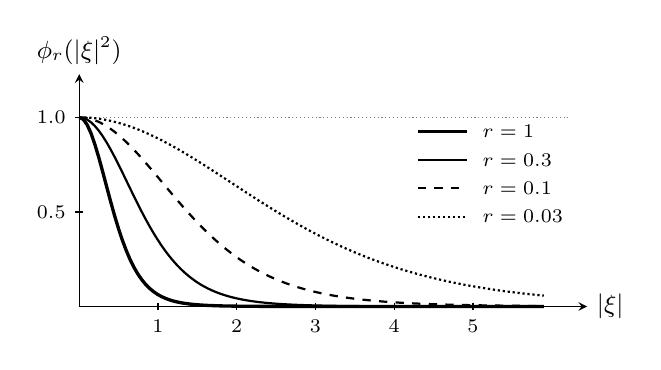
\begin{tikzpicture}[scale=1.0, >=stealth]
    \draw[->] (0,0) -- (6.45,0) node[right, font=\small] {$| \xi |$};
    \draw[->] (0,0) -- (0,2.95) node[above, font=\small] {$\phi_r(| \xi |^2)$};
    \foreach \x in {1,2,3,4,5} \draw (\x,0.05) -- (\x,-0.05) node[below, font=\scriptsize] {$\x$};
    \foreach \y/\lab in {1.20/{0.5}, 2.40/{1.0}}
        \draw (0.05,\y) -- (-0.05,\y) node[left, font=\scriptsize] {$\lab$};
    \draw[gray, densely dotted] (0,2.40) -- (6.20,2.40);
    % r = 1, 0.3, 0.1, 0.03
    \draw[very thick] plot[domain=0:5.9, samples=120] (\x, {2.4*(1+1.0*\x*\x)^(-4)});
    \draw[thick] plot[domain=0:5.9, samples=120] (\x, {2.4*(1+0.3*\x*\x)^(-4)});
    \draw[thick, dashed] plot[domain=0:5.9, samples=120] (\x, {2.4*(1+0.1*\x*\x)^(-4)});
    \draw[thick, densely dotted] plot[domain=0:5.9, samples=120] (\x, {2.4*(1+0.03*\x*\x)^(-4)});
    % 图例 (置于曲线均已衰减的空白区)
    \draw[very thick] (4.30,2.22) -- (4.92,2.22);
    \node[font=\scriptsize, anchor=west] at (5.00,2.22) {$r = 1$};
    \draw[thick] (4.30,1.86) -- (4.92,1.86);
    \node[font=\scriptsize, anchor=west] at (5.00,1.86) {$r = 0.3$};
    \draw[thick, dashed] (4.30,1.50) -- (4.92,1.50);
    \node[font=\scriptsize, anchor=west] at (5.00,1.50) {$r = 0.1$};
    \draw[thick, densely dotted] (4.30,1.14) -- (4.92,1.14);
    \node[font=\scriptsize, anchor=west] at (5.00,1.14) {$r = 0.03$};
\end{tikzpicture}}

% ============ 图 8.5 ============
\newcommand{\drawFigEightFive}{%
\begin{tikzpicture}[scale=1.0, >=stealth]
    % S^*M 边框
    \draw[gray, densely dashed, rounded corners=6pt] (0.30,0.30) rectangle (9.10,4.20);
    \node[gray, font=\small, anchor=north east] at (9.00,4.12) {$S^*M$};
    % Char(P) 曲线
    \draw[thick] (0.70,1.55) .. controls (3.00,1.20) and (5.60,2.90) .. (8.60,2.55);
    \node[font=\small, anchor=west] at (8.62,2.55) {$\operatorname{Char}(P)$};
    % Ell(G)：沿曲线的灰带
    \draw[line width=13pt, gray!22, line cap=round] (0.95,1.52) .. controls (3.05,1.22) and (5.60,2.86) .. (8.05,2.60);
    \node[font=\small] at (4.35,1.02) {$\Ell(G)$};
    % Ell(E)：左端圆盘
    \draw[very thick, gray!60, fill=gray!15] (1.35,1.46) ellipse (0.72 and 0.52);
    \node[font=\small] at (1.35,2.28) {$\Ell(E)$};
    % WF'(B) ∩ Char(P)：右端阴影块
    \fill[gray!45, rounded corners=4pt] (6.70,2.30) rectangle (8.30,2.92);
    \node[font=\small, anchor=south] at (7.50,2.96) {$\WF'(B)\cap\operatorname{Char}(P)$};
    % 后向零双特征线（箭头指向 Ell(E)）
    \draw[->, thick, gray!70] (6.75,2.55) .. controls (5.20,2.72) and (3.10,1.80) .. (2.05,1.55);
    \draw[->, thick, gray!70] (6.90,2.85) .. controls (5.00,3.10) and (2.90,2.20) .. (2.00,1.85);
    \node[font=\small, anchor=west] at (3.85,3.55) {后向零双特征线};
    \draw[->, gray] (3.80,3.42) -- (3.05,2.72);
\end{tikzpicture}}

% ============ 图 8.6 ============
% 例 8.22: P = hD_x - a 的特征集与 H_p 的流
\newcommand{\drawFigEightSix}{%
\begin{tikzpicture}[scale=1.0, >=stealth, line join=round]
    % 坐标轴
    \draw[->] (0.10,2.10) -- (7.55,2.10) node[below right, font=\small] {$x$};
    \draw[->] (4.00,0.15) -- (4.00,4.35) node[above, font=\small] {$\xi$};
    % 特征集 Char_h(P) = { xi = a(x) }, 同时也是 H_p 的一条积分曲线
    \draw[line width=1.1pt,
          postaction={decorate, decoration={markings,
            mark=at position 0.135 with {\arrow{stealth}},
            mark=at position 0.435 with {\arrow{stealth}},
            mark=at position 0.705 with {\arrow{stealth}},
            mark=at position 0.915 with {\arrow{stealth}}}}]
        (0.35,4.02)
        .. controls (1.00,4.18) and (1.50,3.98) .. (2.02,3.60)
        .. controls (2.42,3.34) and (2.68,3.30) .. (2.95,3.22)
        .. controls (3.35,3.10) and (3.62,2.60) .. (3.96,2.10)
        .. controls (4.36,1.52) and (4.86,0.94) .. (5.55,0.80)
        .. controls (6.10,0.70) and (6.58,1.06) .. (7.05,1.46);
    % 标注
    \node[font=\small, anchor=east] (charP) at (1.95,4.62) {$\Char_\hbar(P)$};
    \draw[->, gray] (charP.east) -- (1.28,4.10);
    \node[font=\small, anchor=north] (Hp) at (5.72,0.62) {$H_p$};
    \draw[->, gray] (Hp.north) -- (5.62,0.76);
\end{tikzpicture}}
